
\addcontentsline{toc}{section}{Exercițiul 12}
\section*{12. Formulati in limbaj natural si implementati 5 cereri SQL complexe ce vor utiliza, in ansamblul lor, urmatoarele elemente:}

\vspace{0.5cm}
\begin{itemize}
    \item 
    \begin{lstlisting}
/*
 O cerere nesincronizata care afiseaza
toti chiriasii a caror magazine nu au nicio reclamatie.

-cerere sincronizata cu cel putin 3 tabele
-clauza WITH
*/

WITH Subcerere AS (
 SELECT m.id_chirias
 FROM MAGAZIN m
 LEFT JOIN RECLAMATIE r ON m.id_magazin = r.id_magazin
 WHERE r.id_magazin IS NULL
)
SELECT c.nume_chirias
FROM CHIRIAS c
WHERE c.id_chirias IN (
 SELECT id_chirias
 FROM Subcerere
);
    \end{lstlisting}
    \vspace{0.2cm}
    \begin{figure}[h]
      \centerline{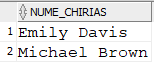
\includegraphics{images/interogare1.png}}
      \caption{ Interogare 1.}
    \end{figure}
    \vspace{0.5cm}

    \item 
    \begin{lstlisting}
/*
 Afisarea tuturor magazinelor a caror mall detine o promovare, selectand
astfel numele magazinului (cu majuscule), data cand incepe campania de promovare
(in format zi-luna-an), data cand se sfarseste campania (in format an-luna-zi), verificandu-se daca este un magazin profitabil (profitul>5000), si daca are un nume lung sau scurt(sa fie de maxim 9 caractere).

-functii cu siruri de caractere/data
-case
*/

SELECT
 UPPER(m.nume_magazin) AS nume_magazin,
 TO_CHAR(p.data_inceput, 'DD-MON-YYYY') AS data_inceput,
 TO_CHAR(p.data_sfarsit, 'YYYY-MM-DD') AS data_sfarsit,
 CASE
 WHEN m.profit_lunar > 5000 THEN 'Profitabil'
 ELSE 'Neprofitabil'
 END AS situatie_profit,
 CASE
 WHEN LENGTH(m.nume_magazin) > 9 THEN 'Nume Lung'
 ELSE 'Nume Scurt'
 END AS lungime_nume
FROM MAGAZIN m
JOIN MALL ma ON m.id_mall = ma.id_mall
JOIN PROMOVARE p ON ma.id_promovare = p.id_promovare
WHERE ma.id_promovare IS NOT NULL;
    \end{lstlisting}
    \vspace{3cm}
    \begin{figure}[h]
      \centerline{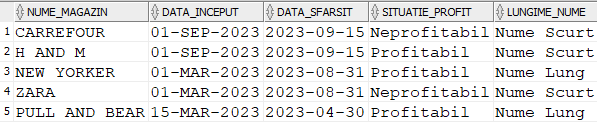
\includegraphics{images/interogare2.png}}
      \caption{ Interogare 2.}
    \end{figure}
    \vspace{0.5cm}

    \item 
    \begin{lstlisting}
/*
 Afisarea tuturor magazinelor care au profitul lunar mai mare de 5000.

 -Functii grup ( GROUP BY, HAVING)
*/
SELECT nume_magazin, SUM(profit_lunar) AS profit_total
FROM MAGAZIN
GROUP BY nume_magazin
HAVING SUM(profit_lunar) > 5000
    \end{lstlisting}
    \vspace{0.2cm}
    \begin{figure}[h]
      \centerline{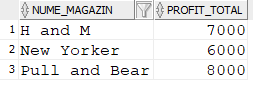
\includegraphics{images/interogare3.png}}
      \caption{ Interogare 3.}
    \end{figure}
    \vspace{0.5cm}


    \item 
    \begin{lstlisting}
/*
Sa se afiseze toti paznicii (id-ul, numele_angajatului) si firma la care lucreaza care au o norma intreaga.

-subcerere nesincronizata in FROM
*/

SELECT p.id_paznic, a.nume_angajat, f.nume_firma
FROM (SELECT * FROM PAZNIC WHERE norma = 'Norma intreaga') p, FIRMA f, ANGAJAT a
WHERE p.id_firma = f.id_firma
AND p.id_angajat = a.id_angajat
    \end{lstlisting}
    \vspace{0.2cm}
    \begin{figure}[h]
      \centerline{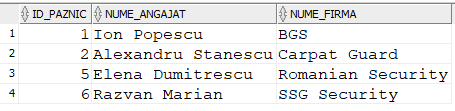
\includegraphics{images/interogare4.png}}
      \caption{ Interogare 4.}
    \end{figure}
    \vspace{0.5cm}

    \item 
    \begin{lstlisting}
/*
Sa se afiseze toate mall-urile, cu campaniile de promovare (numele mall-ului, numele campaniei, data de incepere, si data de sfarsit) In cazul in care mall-ul nu are campanie se va afisa "Fara campanie", iar la data de inceput si sfarsit "Informatie indisponibila"

-DECODE
*/
SELECT m.nume_mall, NVL(p.nume_campanie, 'Fara campanie') AS nume_campanie,
 DECODE(p.data_inceput, NULL, 'Informatie indisponibila', TO_CHAR(p.data_inceput, 'DDMM-YYYY')) AS data_inceput,
 DECODE(p.data_sfarsit, NULL, 'Informatie indisponibila', TO_CHAR(p.data_sfarsit, 'DDMM-YYYY')) AS data_sfarsit
FROM MALL m
LEFT JOIN PROMOVARE p ON m.id_promovare = p.id_promovare;
    \end{lstlisting}
    \vspace{0.2cm}
    \begin{figure}[h]
      \centerline{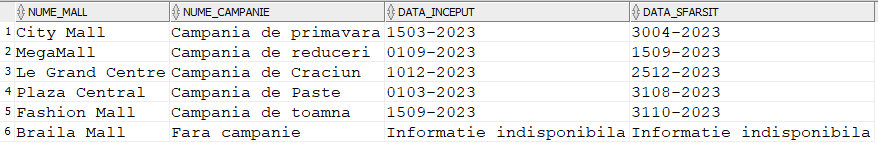
\includegraphics{images/interogare5.png}}
      \caption{ Interogare 5.}
    \end{figure}
    \vspace{0.5cm}
\end{itemize}
